% just like python and another other programming language
% we must load our packages and setup the document

\documentclass[man, 12pt, donotrepeattitle, floatsintext]{apa7} % I want to load the apa6 features

\usepackage[utf8]{inputenc}
\usepackage{amsmath, amssymb}
\usepackage{graphicx}
\usepackage{url}
\usepackage{float}

\usepackage{longtable} % Required for the longtable environment
\usepackage{array} % Required for custom column specifications
\usepackage{calc} % Required for calculations
\usepackage{ragged2e} % Required for \raggedright in column specification
\usepackage{booktabs} % Required for \toprule, \midrule, \bottomrule



\usepackage[style=apa, doi=true, backend=biber]{biblatex}
\DeclareLanguageMapping{american}{american-apa}
\addbibresource{sources.bib}

% this section contains everything needed for titling and headers
\title{Examining Housing Instability Trends and the Moderating Impacts of the Covid-19 Eviction Moratorium in San Diego County}
\shorttitle{Housing Instability}
\leftheader{Prosser, Lona}
\author{Kaye Prosser, Andrew Lona}
\affiliation{{University of California, San Diego}}
\authornote{Special thanks to our capstone advisors, Dr. Jennifer Nations and Julie Wartell.}
% the following contains our abstract/aka the draw
%\keywords{keyword1, keyword2}
%\abstract{ABSTRACT TEXT HERE}


% this has the meat and potatoes of our paper
\begin{document} % can ignore this, just let's LaTeX know we are beginning our main writing
\maketitle % needed to create the title page (generated from the stuff above)
\tableofcontents % adds a table of contents
\vspace{3.5in}
\url{https://github.com/AndyLAndrew/Homelessness_Hub_MS_CSS_Capstone}
\pagebreak % adds a page break







% this is the body
\section{Contributions}

\textbf{Kaye Prosser}: In my role I worked specifically with the Eviction data providing spatial information on Evictions across San Diego County.  

\begin{enumerate}
    \item I conducted spatial analysis of eviction data, exploring patterns and relationships within specific locations. By mapping evictions across moratorium periods in San Diego County, we gained insights into the changes occurring during Covid19.
    \item I played a role in cleaning and organizing the eviction data. This process ensured its reliability, structure, and integrity, making it suitable for further analysis by the team and others. 
    \item I performed geocoding on the eviction data, adding precise location information. By integrating this data with other geographic layers, such as census ZIP code boundaries, and developed accurate eviction rates for each period.
\end{enumerate}

These efforts enhanced our understanding of eviction patterns over the Covid19 Moratorium in San Diego County. The insights generated from our work aided decision-making processes, while the cleaning, organization, and geocoding of the data ensured its reliability and facilitated integration with other geographic layers for comprehensive analysis.

\textbf{Andrew Lona}: In my role I worked specifically with the CIE data to create models that would best explain eviction patterns over the San Diego County Covid19 Moratorium.

\begin{enumerate}
    \item I extracted, processed, and analyzed specific variables within the CIE dataset.
    \item Cleaning data: I meticulously reviewed and resolved inconsistencies, missing values, and outliers, ensuring the integrity and quality of the CIE data.
    \item Data management: I implemented efficient storage and organization strategies for CIE data, enabling easy access and streamlined analysis for the team.
    \item Building regression models: Leveraging statistical modeling and machine learning techniques, I developed robust regression models to uncover relationships, predict outcomes, and provide valuable insights from the CIE data.
\end{enumerate}

Overall, my contributions focused on working with CIE data, ensuring data cleanliness, implementing effective data management practices, and building reliable models. These efforts enhanced data accuracy, accessibility, and facilitated informed decision-making in our research.

\textbf{Joined}:
	The overall design, hypothesis, question, topic decision and all writing was worked on as a team. Together we also worked toward understanding the patterns that connected both the CIE data and the Eviction data. 







\section{Introduction} % you can make a section and add a title in the {}


Across the nation, it is estimated that there is a deficiency of approximately 7 million reasonably priced residences for households with extremely low income \parencite{Kuntz2019}. In California alone that deficiency comes to 1 million homes. Families are contending for a progressively scarce selection of reasonably priced homes, leading to elevated housing expenses and an augmented financial burden on lower- and middle-income households. Due to the insufficient growth of wages and public support in contrast to the escalating cost of housing and other essential expenses, numerous households encounter ongoing uncertainty in their housing situation and may find themselves trapped in this predicament for a significant portion of their lives, even without experiencing homelessness. According to a January survey conducted by the Census Bureau, over 33\% of American adults continue to face difficulties in meeting essential household expenses, with 11\% reporting insufficient food availability in the previous week \parencite{Vesoulis2021}. Housing instability occurs in cities across the county, but is more likely to result in homelessness in cities such as San Diego, where income inequality and housing prices are high. According to the 2018 Housing Action Plan report \footnote{Housing Action Plan: \url{https://www.sandiego.gov/sites/default/files/housing_plan_final.pdf}}, by the city of San Diego, the Area Median Income (AMI) in San Diego stood at around \$79,000. However, the total number of rental units available countywide that are affordable at that income level fell below 45,000. These struggles especially affect those who have a record of systemic discrimination in the United States. People of color have continued to grapple with these barriers in society and the pandemic has only intensified these disparities. By April 2020, job losses attributable to the pandemic were already affecting a significant proportion of the adult population, with 32 percent of Black adults and 41 percent of Latinx adults experiencing unemployment, in contrast to just 24 percent of white adults \parencite{Lake2022}.  Understanding these factors is very important for our exploration, and can support findings of spatial patterns of eviction in San Diego County. 

We address these issues asking two questions: What factors influenced housing instability before, during, and after Covid-19 eviction moratoriums\footnote{San Diego Eviction Moratorium Summary} in San Diego county? If any, which trends could best explain these differences across the county? In order to answer these questions we are using two approaches for estimating housing instability. The first is too view eviction rates geographically across Moratorium periods for the Covid-19 pandemic time frame: 1 = “pre-moratorium", 2 = “moratorium in place" and 3 = "post-moratorium"\footnote{Throughout this paper these periods will also be referred to as before, during, and after}. The second is to run regression models on variables of housing instability. However, measuring housing instability and evictions is very difficult due to filing inconsistencies and the lack of available data. Due to this we pulled from two data sources that provided different types of insights into housing instability in San Diego county. Both data sets include a long enough time series that we are able to investigate a period of two years prior to the pandemic, two years during and 9 months after the moratorium.

The two data sets we will be exploring consist of Sheriff Department lock-out eviction orders and the Community Information exchange(CIE)\footnote{This data will be referred to as CIE through the paper} database containing information from 2-1-1 calls\footnote{More information on CIE and 2-1-1 can be found here: https://ciesandiego.org/what-is-cie/}. While exploring these data sets we began to ask another question. Was there any impact on 2-1-1 calls regarding housing insecurity and eviction lock-outs due to the COVID-19 Moratorium? While programs for aid during the pandemic such as, The Coronavirus Aid, Relief, and Economic Security (CARES) Act\footnote{https://home.treasury.gov/policy-issues/coronavirus/about-the-cares-act}, were essential they also fell short; requiring emergency action due to needs remaining high \parencite{Lake2022}. The CIE data is a good source for this type of information as it contains the 2-1-1 infrastructure which serves as a host for a comprehensive resource database. It contains listings of service offerings, eligibility criteria, and intake information for health, human, and social services providers. With this data set we will be able to obtain our variables of housing instability from our own local ZIP codes in San Diego County. Both data sets include a long enough time series that we are able to investigate a period of 26 months prior to the pandemic, 25 months during and 9 months after the moratorium.

When we include CIE data we will be able to pinpoint instabilities that might explain descriptors that ensure housing security. We will be using Census ZIP codes, also referred to as ZCTA, to spatially analyze our data. While proving causation is not possible in this study, we seek to understand the potential relationships between eviction rates before, during and after the moratorium while also including the instability types. Our variables for instability contain: housing need, medical, utility and eviction. Our control variables include: race, household size, age, and localized poverty rate. In our models we will take into account the time periods before, during and after moratorium. This exploration gives us insight to the variables that best explain the rate of evictions in any of these periods. Choosing eviction data is important to this project because of the ability to understand evictions spatially. The decision to explore CIE data assisted in our ability to find variables which help explain the spatial information of change before, during and after the moratorium by ZIP. We used two logistic regression models in order to help explain the changes in prediction power of housing precarity within CIE when accounting for changes before, during, and post-moratorium. 

It is our presumption that there will be a difference before, during and after the pandemic moratorium. When starting this research we expected to see a decrease in evictions during the moratorium period followed by a large spike after the moratorium is lifted. We hypothesized that there would be no change in areas such as Coronado, La Jolla, Encinitas, Carlsbad and other coastal cities. Additionally, we noted that while the moratorium was used to  protect tenants there would be a decrease in calls for housing needs but an increase in utility or health needs due to the pandemic.

This study utilized GIS mapping and statistical modeling techniques to examine the spatial patterns of change during the COVID-19 moratorium regarding housing instability and evictions in San Diego County. The dependent variables of interest were housing needs and utilities needs, both representing binomial outcomes indicating the level of housing precarity over time (by date) and space (by ZCTA). We fitted four binomial logistic regression models, with two models for each outcome. The GIS mapping analysis helped visualize the spatial distribution of evictions before, during and after the moratorium; while the logistic regression models allowed us to assess the factors influencing these outcomes. By combining these approaches, we gained insights into the spatial patterns and determinants of evictions and housing precarity temporally.

After mapping the eviction data and completing regression models for comparison from the CIE data, we found that there is a definitive difference between before, during and after the moratorium. We found that a decrease of evictions was prevalent during and after the moratorium when compared with before. While we would assume the moratorium would ensure no evictions occurred, this was not the case. It is evident through our results that evictions continued to occur even when the moratorium was in place. However, it is also important to note that there is an increase happening between during and after the moratorium. To further understand this change, we calculated the rate of change between periods. This showed how much the eviction rate increased or decreased between Periods and gave us a closer look at the changes during and after the moratorium had ended. 


\section{Background}


Housing insecurity, housing precarity, the threat of displacement, and eviction are important topics because they directly affect individuals, families, and communities. The effects of housing instability can advance homelessness, increase stress, and disrupt social networks. These consequences could then generate psychological instability proving to be a direct effect of one's physical stability \parencite{DesmondKimbra2015EFHH}. Additionally, when we consider finances, the increasing housing-cost burdens people dramatically and this too increases housing instability \parencite{KangSeungbeom2019WLHB}. The continuation of physical, mental and home instabilities worsen existing inequalities and contribute to a cycle of poverty \parencite{DesmondKimbra2015EFHH}. When these instabilities lead to eviction, individuals can find themselves in a “downward move”, meaning they typically relocate to disadvantaged neighborhoods and/or substandard housing (Desmond. 2018). Understanding these issues is essential for developing effective strategies to address housing affordability, promote housing stability, and ensure access to safe and affordable housing for all.

While it is important for us to understand the underlying causes of eviction, there is also benefit to doing a geographic analysis. Spatial patterns of evictions and their associations with poverty, race, and ethnicity indicate that these phenomena are not haphazard \parencite{Medina2020102804}. Insufficient availability of affordable housing heightens the likelihood of eviction, leading to the displacement of tenants and making it more challenging to find alternative housing options \parencite{NelsonKyle2021SCaS}. This often results in tenants being compelled to relocate to areas outside the city or end up living on the streets. Housing insecurity and eviction rates can vary significantly across different regions, neighborhoods, and communities. At a smaller scale, within particular housing markets, landlords have the ability to concentrate specific classes of tenants in particular neighborhoods and types of housing using a phenomenon known as reverse selection \parencite{NelsonKyle2021SCaS}. In this process, landlords possess the market influence to choose tenants rather than tenants having the autonomy to select landlords and neighborhoods. The phenomenon of reverse selection can play a role in shaping the spatial dynamics of eviction within racially segregated neighborhoods, where various forms of disadvantage are also concentrated in specific geographical areas \parencite{NelsonKyle2021SCaS} This geographic analysis allows for a deeper understanding of the spatial distribution of eviction.

Studying eviction patterns and trends is challenging without accurate data. We are fortunate to have obtained these records for San Diego County via a public records request. Persisting challenges include the presence of informal evictions that remain unrecorded in eviction court records and databases\parencite{Cheng2021}. Furthermore, the absence of a statewide mandate for landlords to submit eviction notices contributes to the limited availability of comprehensive data. Additionally, varying enforcement approaches across different cities that track eviction data further complicate the accuracy and comprehensiveness of the information that is accessible. California state law safeguards eviction court records from public visibility, which safeguards tenant privacy but hampers the effectiveness of addressing the eviction crisis. It is because of these barriers that we are using two different approaches for this study. By using Sheriff Department lock-out eviction orders and CIE data we will be able to analyze counts of eviction with demographic and other socioeconomic indicators that may explain housing instability all while upholding anonymity. 

These evictions are especially important for us to study because of the time frame that they occur in. On September 4th, 2020, the Centers for Disease Control and Prevention (CDC) implemented a nationwide suspension on residential evictions for nonpayment of rent. This measure mandated renters to complete a declaration form confirming their eligibility based on certain criteria. The CDC acknowledged the importance of housing stability in safeguarding public health, as homelessness increases the risk of individuals residing in crowded spaces such as shelters, heightening the chances of COVID-19 transmission \parencite{Lake2022}. This suspension followed the expiration of the CARES Act on July 24, 2020; over a month and a week after the initial wave of 30-day eviction notices. During this period of reduced protection, numerous cities witnessed a notable surge in eviction filings by late August, with some experiencing increases as high as 118 percent above average(Lake, 2020). Despite the CDC's intervention, local courts continued to process evictions for numerous families. Moreover, the Trump administration issued guidance in October that added to the difficulties faced by struggling renters. This guidance allowed landlords to challenge tenants' eligibility declaration, even though tenants already provided such declarations under the penalty of perjury, enabling landlords to proceed with eviction filings. These eviction protections also had differing start and end dates due to state, county and cities all having separate moratorium time frames. If a city or county had not enacted their own ordinance then the state mandate would control restrictions on eviction. The State of California implemented a ban on residential evictions, which was in effect from March 1, 2020, until September 30, 2021. This State law\footnote{California Eviction Moratorium: https://www.contracosta.ca.gov/DocumentCenter/View/65638/Eviction-Moratorium} also prohibited certain evictions for nonpayment of rent from October 1, 2021, through March 31, 2022, in cases where landlords failed to cooperate with tenants in seeking governmental financial assistance. Additionally, from May 22, 2022 to September 30, 2022, local law in San Diego County prohibited "no-fault" eviction cases\footnote{Information about overall evictions can be found here: https://selfhelp.courts.ca.gov/eviction} within the city. This meant that landlords were unable to evict tenants for reasons unrelated to nonpayment of rent or violation of lease agreements. For our study we will be concentrating on the county time frame as follows: before moratorium January 1, 2018 to February 28th, 2020, during moratorium March 1, 2020 to March 31, 2022, and after the moratorium April 1st, 2022 to December 31st 2022.






\section{Data and Methods}

This study employed two methods of analysis. These methods included GIS mapping and advanced statistical modeling techniques to comprehensively examine the spatial patterns and underlying factors driving housing instability and evictions during the COVID-19 moratorium in San Diego County. With a focus on housing needs and utilities needs as the dependent variables, which were indicative of the level of housing precarity over time (by date) and space (by ZCTA), we crafted four binomial logistic regression models to gain a deep understanding of the influences on these outcomes. The integration of GIS mapping analysis played a pivotal role in visually representing the spatial distribution of evictions before, during, and after the moratorium. Through the strategic amalgamation of these innovative approaches, we not only unraveled the complex temporal dynamics and spatial patterns of evictions and housing precarity but also illuminated the underlying mechanisms driving these phenomena. This methodology provided invaluable insights into the multifaceted nature of the housing crisis during the COVID-19 moratorium, shedding light on critical factors and spatial variations that contribute to a deeper understanding of the issue.

\subsection{Forced Evictions Data}
The data and methods used in this section of the study involved the following steps. First, we obtained records of court-ordered forced eviction lockouts, referred to in this paper as eviction data, for the years 2018 to 2022. These records contained information such as eviction status, ZIP code, street address, city, and date. These records were provided by the Homelessness Hub at the University California of San Diego. 

Next, we converted the obtained forced eviction-lockout records from PDF format into a  data frame for easier manipulation and analysis. This conversion allowed us to organize the data in a structured format suitable for further processing. Afterwards, we proceeded to clean and geocode the data. This involved removing any inconsistencies or errors in the data, fixing typos, and assigning geographical coordinates to the records based on their addresses through using Esri ArcGIS Pro Software. The geocoding process transformed the addresses to a location on the earth surface; ensuring that each eviction record could be associated with a specific location.

Once the data was cleaned and geocoded, we spatially joined the eviction counts to the ZIP codes. To further analyze the impact of the COVID-19 pandemic on eviction rates, we utilized the dates associated with each eviction record to group them into three periods: before, during, and after the pandemic. This allowed us to examine any variations in eviction rates during these different time periods. In addition to the eviction data, we obtained records of San Diego County census ZIP codes, also known as ZCTAs (ZIP Code Tabulation Areas). This layer included information on rental households occupancy for the years 2018 - 2021. While we did not have 2022 data available for the number of rental households, we felt that the count for 2021 would be adequate.

We then joined the eviction data with the census ZCTA data and calculated eviction rates by dividing the eviction counts by the number of rental households for each year within each period, then multiplied by 1000. To account for differing numbers of months in each period and normalize the data, we divided the rates by the number of months in each period.

Definition: For each period ($p$) for each Zip/ZCTA ($z$):
$$evictionsrate = \frac{(evictionscounts_{zp}/rentalhouseholdoccupancy_{zp} * 1000)}{month_{p}}$$

It is important to refer to the descriptive statistics(see table 1) for further details on these calculations. 


\begin{figure}[H]
  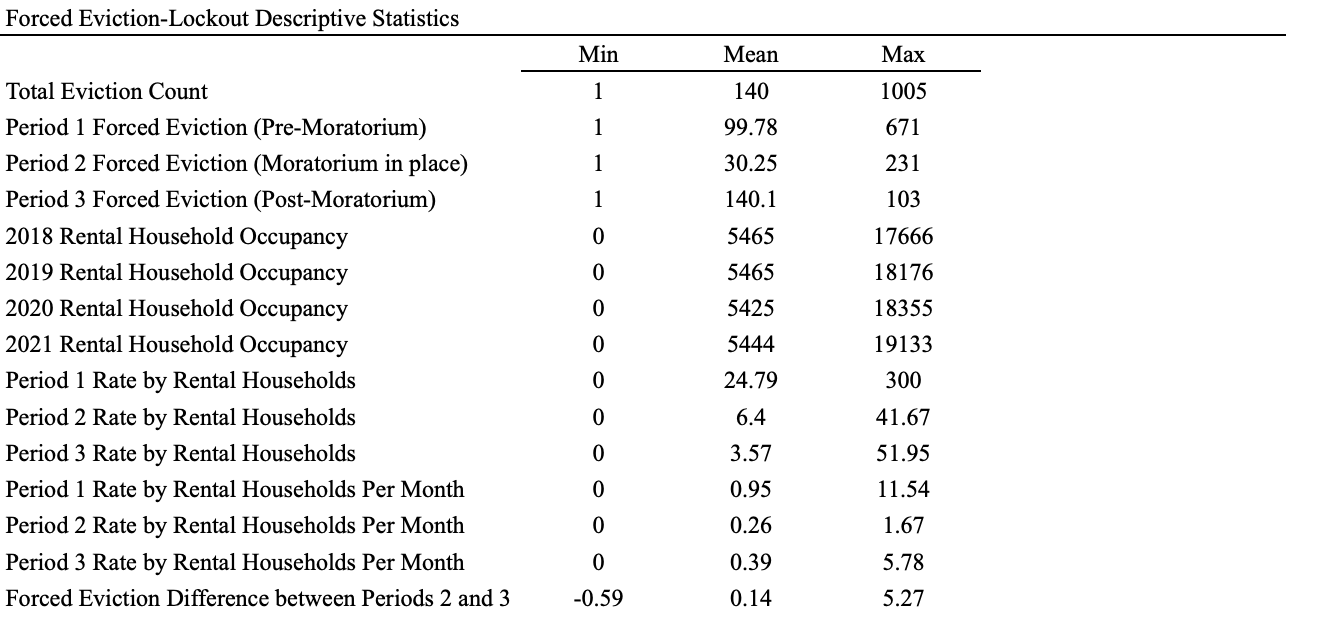
\includegraphics[width=\linewidth]{figures/Table_1_FEviction_DescriptiveSTATS.png}
  \caption{Descriptive Statistics for Eviction Lockout Data}
  \label{fig:descriptive_stats_evictions}
\end{figure}


Furthermore, we uploaded the processed data to ArcGIS for spatial analysis and mapping. This allowed us to visualize and analyze the geographical distribution of eviction rates across the study area. During the mapping process, it became apparent that outliers were present in the data, which significantly skewed the results. To address this issue, we filtered out ZIP codes with less than 20 households, as these outliers had a disproportionate impact. Additionally, when examining the rate of change, we filtered out zero values as they represented extreme outliers.



\begin{figure}[H]
  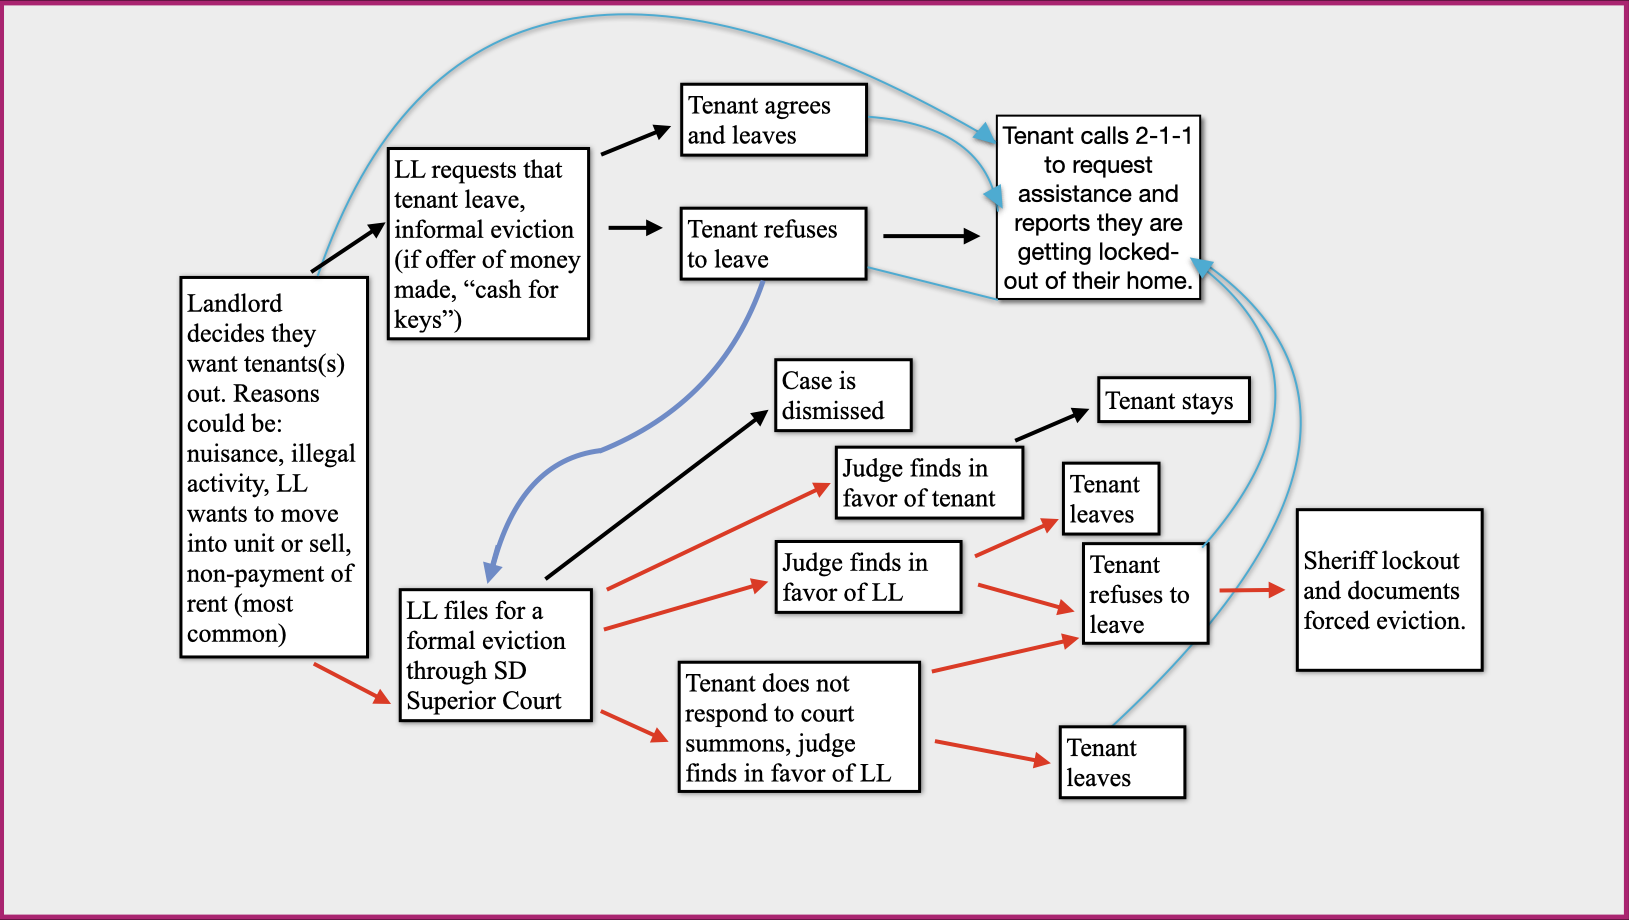
\includegraphics[width=\linewidth]{figures/housing_precarity_tree.png}
  \caption{Illustration of housing precarity ties.}
  \label{fig:housing_precarity_tree}
\end{figure}


To further analyze the temporal dynamics of evictions, we calculated the rate of change between each period. This rate of change provides insights into the direction and magnitude of eviction trends, enabling us to identify periods characterized by changes or stability in eviction rates. By examining the rate of change, we can obtain a clear understanding of how much evictions have changed or stabilized across San Diego County before, during, and after eviction moratoriums were in place. 



\subsection{CIE Demographics Data}

We used the 2018-2022 Community Information Exchange\footnote{CIE for short} demographics data consisting of any San Diego County 2-1-1 callers determined to have instability or unaddressed needs. The CIE itself is a network of partners/organizations whom all provide assistance in some form to people within San Diego County, this involves hospitals, resource centers, homeless shelters, and health insurance providers. Callers requesting information or assistance when calling the 2-1-1 line will be directed towards network partners such as San Ysidro Health or the North County LRBTQ Resource Center where they are then assessed using shared language across all CIE partners to determine their risk and level of need. Throughout this process, per each caller, a longitudinal record of their assessments and referrals is kept and shared throughout the CIE network to assist the current provider with providing the correct future referrals to other providers or update need assessments if needed. It is from here where our four needs; Housing, Utilities, Evictions, and Medical\footnote{Each need is a binary Yes or No/Not Known outcome.}, originate within our dataset. All callers are determined by a network provider to express a need, but each caller can have any combination of the four based on the assessment answers provided.\footnote{CIE will not provide us with the questions used to determine each need.} \parencite{CIE_webpage}.

 After accounting for missing data, we have a total of 20,282 observations between the dates of 2018-01-01 - 2022-12-30. Our dependent variables of interest are: housing needs and utilities needs, both binomial outcomes which can reflect the status of housing instability per each recorded call within time (by date), and space (by ZCTA). Two other outcomes; eviction needs and medical needs, are omitted from this analysis due to no measurable change in outcome, for both have "No/Not Known" for all but < 30 observations. We unfortunately do not have an explanation from CIE on why both eviction needs and medical needs seem to have so few "Yes" entries by providers. To account for factors known to influence housing instability; gender, age, and race/multi-ethnicity\footnote{Race/ethnicity is factored as a categorical within both models.} have been added as base terms to the logistic regression model, as binomial, ordinal, and categorical variables respectively. In order to control for the rate of poverty by ZCTA, the accompanying ZIPcodes per observation were matched with their corresponding ZCTA value, then each observation was matched with their respective poverty rate as defined\footnote{Zip to ZCTA mapper used: \url{https://udsmapper.org/zip-code-to-zcta-crosswalk/}}:

For every $Year$ within each $ZCTA$, calculate the poverty rate utilizing the $Population$ number and number in $Poverty$ defined as:
$$Poverty Rate = \frac{{\text{Poverty}_{ZCTA, Year}}}{{\text{Population}_{ZCTA, Year}}} * 100$$

	To create our models, we fitted two binomial logistic regression models each for both of our outcomes for our hypothesis. Assuming that both Utilities and Housing needs are independent, our $H_{0}$: states the Moratorium period had no effect on the change in need for CIE-determined 2-1-1 callers, while our $H_{1}$ states: the Moratorium period does have an effect on the change in need for CIE-determined 2-1-1 callers, as expressed:
$$Precarity Identifier{H_0} = \beta_0 + \beta_1 \cdot Accounts + \beta_2 \cdot Poverty Rate + \epsilon$$
$$Precarity Identifier(H_1) = \beta_0 + \beta_1 \cdot Accounts + \beta_2 \cdot Poverty Rate + \beta_3 \cdot Moratorium Period + \epsilon$$
In order to test the in-sample model fit of both the null and alternative models, we've decided to focus on the Akaike Information Criterion which is defined as: $\text{AIC} = -2 \ln(L) + 2k\:$\footnote{for AIC and Log Likelihood, k is the number of parameters}. The AIC is a useful indicator of in-sample model fit as adds an additional term, $2k$ to the log likelihood function $-2 \ln(L)$ used to provide a simple in-sample model fit score. The log likelihood, while a useful metric, only provides us with the likelihood of the data given the model as defined\footnote{Moratorium Period is removed for $H_{0}$ otherwise the formulas are the same.}:

$L(H1) = \prod_{i=1}^{n} \left(\frac{1}{1 + e^{-(\beta_0 + \beta_1 \cdot Accounts_i + \beta_2 \cdot PovertyRate + \beta_3 \cdot MoratoriumPeriod_{k})}}\right)^{PrecarityIdentifier_{k}} \times \left(1 - \frac{1}{1 + e^{-(\beta_0 + \beta_1 \cdot Accounts_i + \beta_2 \cdot PovertyRate + \beta_3 \cdot MoratoriumPeriod_{k})}}\right)^{(1 - PrecarityIdentifier_{k})}$
 
	As expressed, the likelihood of the hypothesis is determined by the product of the probability of our predictors times their inverse probability (one minus) for all the observations in our CIE dataset. This will provide us with an estimate likelihood of our hypothesis given the data presented. We take the log of such a likelihood for mathematical convenience, providing us with the log-likelihood of our model. With $2k$ of AIC added as an extra term, we can account for the added complexity of our multiple covariates and thus punish the score accordingly based on the number of $k$. We are not looking at the Bayesian information criterion (BIC) for our model comparison as it too heavily punishes the model for its complexity. We have a large set of categorical predictors from race/ethnicity which would over-inflate $k$ past what BIC is ideal to use.


After creating and scoring both our alternative and null models testing the interaction of the San Diego County moratorium on both measures of need\footnote{needs will be referring to both housing and utilities needs.}, a repeated K-Fold cross validation process was conducted to account for both the bias of our model which can arise when fitting a high complexity model over a low $n$ dataset. K-Fold itself allows us to randomly split all of our CIE observations into chunks by $k$, which is 50. For each fold of k, we fit both models over the observations outside of the k group and test against the left out observations (in the group). After this process is completed, we then take the average performance across all folds. A repeated k-fold allows us to further perform k-folding by repeating this process and taking the mean across all scores, we have picked five repeats due to the number of observations and available compute performance:\footnote{While confusing, we are using K for these two formulas as standard practice. k is the number of Folds per r (repeat), totals are K and R respectively.}
$$\text{CV}(K=50, R=5) = \frac{1}{R} \sum_{r=1}^{R} \left( \frac{1}{K} \sum_{k=1}^{K} \text{Loss}(k, r) \right) $$

Lastly, in order to compare how well the models perform following cross validation, the average area-under-the-curve scores are computed by predicting the outcomes of need based on the left out data for each fold and repeat. Utilizing these predictions, we can generate a confusion matrix when comparing to the true outcomes of need, and calculate the area under the curve for our models, a useful indicator for viewing the performance differences between the null and alternative hypotheses.
$$AUC = \frac{1}{K \times R} \sum_{r=1}^{R} \sum_{k=1}^{K} AUC_{r,k}$$
	

\begin{longtable}[]{@{}
  >{\raggedright\arraybackslash}p{(\columnwidth - 8\tabcolsep) * \real{0.3824}}
  >{\centering\arraybackslash}p{(\columnwidth - 8\tabcolsep) * \real{0.1544}}
  >{\centering\arraybackslash}p{(\columnwidth - 8\tabcolsep) * \real{0.1544}}
  >{\centering\arraybackslash}p{(\columnwidth - 8\tabcolsep) * \real{0.1544}}
  >{\centering\arraybackslash}p{(\columnwidth - 8\tabcolsep) * \real{0.1544}}@{}}
\caption{Descriptive Statistics for CIE Data Grouped by Moratorium Period}\tabularnewline
\toprule\noalign{}
\begin{minipage}[b]{\linewidth}\raggedright
\end{minipage} & \begin{minipage}[b]{\linewidth}\centering
1(N=10922)
\end{minipage} & \begin{minipage}[b]{\linewidth}\centering
2(N=7472)
\end{minipage} & \begin{minipage}[b]{\linewidth}\centering
3(N=1888)
\end{minipage} & \begin{minipage}[b]{\linewidth}\centering
Total (N=20282)
\end{minipage} \\
\midrule\noalign{}
\endfirsthead
\toprule\noalign{}
\begin{minipage}[b]{\linewidth}\raggedright
\end{minipage} & \begin{minipage}[b]{\linewidth}\centering
1 (N=10922)
\end{minipage} & \begin{minipage}[b]{\linewidth}\centering
2 (N=7472)
\end{minipage} & \begin{minipage}[b]{\linewidth}\centering
3 (N=1888)
\end{minipage} & \begin{minipage}[b]{\linewidth}\centering
Total (N=20282)
\end{minipage} \\
\midrule\noalign{}
\endhead
\bottomrule\noalign{}
\endlastfoot
\textbf{Housing Needs} & & & & \\
~~~Mean (SD) & 0.470 (0.499) & 0.420 (0.494) & 0.305 (0.460) & 0.436
(0.496) \\
~~~Range & 0.000 - 1.000 & 0.000 - 1.000 & 0.000 - 1.000 & 0.000 -
1.000 \\
\textbf{Utilities Needs} & & & & \\
~~~Mean (SD) & 0.448 (0.497) & 0.300 (0.458) & 0.194 (0.396) & 0.370
(0.483) \\
~~~Range & 0.000 - 1.000 & 0.000 - 1.000 & 0.000 - 1.000 & 0.000 -
1.000 \\
\textbf{At Risk Of Losing Housing} & & & & \\
~~~Mean (SD) & 0.106 (0.308) & 0.121 (0.326) & 0.160 (0.367) & 0.116
(0.321) \\
~~~Range & 0.000 - 1.000 & 0.000 - 1.000 & 0.000 - 1.000 & 0.000 -
1.000 \\
\textbf{Financial Barriers} & & & & \\
~~~Mean (SD) & 0.903 (0.296) & 0.902 (0.297) & 0.880 (0.325) & 0.900
(0.300) \\
~~~Range & 0.000 - 1.000 & 0.000 - 1.000 & 0.000 - 1.000 & 0.000 -
1.000 \\
\textbf{Eviction Pay Quit} & & & & \\
~~~Mean (SD) & 0.098 (0.297) & 0.073 (0.260) & 0.104 (0.305) & 0.089
(0.285) \\
~~~Range & 0.000 - 1.000 & 0.000 - 1.000 & 0.000 - 1.000 & 0.000 -
1.000 \\
\textbf{Gender} & & & & \\
~~~Mean (SD) & 0.697 (0.459) & 0.601 (0.490) & 0.594 (0.491) & 0.652
(0.476) \\
~~~Range & 0.000 - 1.000 & 0.000 - 1.000 & 0.000 - 1.000 & 0.000 -
1.000 \\
\textbf{Age Group} & & & & \\
~~~Mean (SD) & 3.351 (1.543) & 3.217 (1.588) & 2.991 (1.694) & 3.268
(1.578) \\
~~~Range: 0=19\&under | 8=90+ & 0.000 - 8.000 & 0.000 - 8.000 & 0.000 - 8.000 & 0.000 -
8.000 \\
\textbf{Race, Multiethnicity} & & & & \\
~~~African American/ Black & 2584 (23.7\%) & 1352 (18.1\%) & 377
(20.0\%) & 4313 (21.3\%) \\
~~~Alaska Native/ Native Indian & 126 (1.2\%) & 108 (1.4\%) & 21 (1.1\%)
& 255 (1.3\%) \\
~~~Asian/ Pacific Islander/ Hawaiian & 618 (5.7\%) & 525 (7.0\%) & 148
(7.8\%) & 1291 (6.4\%) \\
~~~Bi-Racial/ Multi-Racial & 531 (4.9\%) & 312 (4.2\%) & 110 (5.8\%) &
953 (4.7\%) \\
~~~Hispanic/Latino & 171 (1.6\%) & 121 (1.6\%) & 36 (1.9\%) & 328
(1.6\%) \\
~~~Other & 486 (4.4\%) & 579 (7.7\%) & 133 (7.0\%) & 1198 (5.9\%) \\
~~~White/ Caucasian & 3913 (35.8\%) & 2499 (33.4\%) & 663 (35.1\%) &
7075 (34.9\%) \\
~~~White/ Hispanic/ Latino & 2493 (22.8\%) & 1976 (26.4\%) & 400
(21.2\%) & 4869 (24.0\%) \\
\textbf{Language} & & & & \\
~~~Arabic & 90 (0.8\%) & 132 (1.8\%) & 19 (1.0\%) & 241 (1.2\%) \\
~~~Cambodian & 2 (0.0\%) & 1 (0.0\%) & 1 (0.1\%) & 4 (0.0\%) \\
~~~Cantonese & 2 (0.0\%) & 1 (0.0\%) & 0 (0.0\%) & 3 (0.0\%) \\
~~~Chinese & 1 (0.0\%) & 4 (0.1\%) & 3 (0.2\%) & 8 (0.0\%) \\
~~~English & 8755 (80.2\%) & 5347 (71.6\%) & 1527 (80.9\%) & 15629
(77.1\%) \\
~~~Farsi & 37 (0.3\%) & 45 (0.6\%) & 15 (0.8\%) & 97 (0.5\%) \\
~~~Italian & 0 (0.0\%) & 2 (0.0\%) & 0 (0.0\%) & 2 (0.0\%) \\
~~~Korean & 2 (0.0\%) & 2 (0.0\%) & 1 (0.1\%) & 5 (0.0\%) \\
~~~Mandarin & 3 (0.0\%) & 4 (0.1\%) & 1 (0.1\%) & 8 (0.0\%) \\
~~~Other & 565 (5.2\%) & 449 (6.0\%) & 58 (3.1\%) & 1072 (5.3\%) \\
~~~Portuguese & 1 (0.0\%) & 8 (0.1\%) & 4 (0.2\%) & 13 (0.1\%) \\
~~~Russian & 10 (0.1\%) & 10 (0.1\%) & 5 (0.3\%) & 25 (0.1\%) \\
~~~Somali & 3 (0.0\%) & 1 (0.0\%) & 2 (0.1\%) & 6 (0.0\%) \\
~~~Spanish & 1395 (12.8\%) & 1386 (18.5\%) & 228 (12.1\%) & 3009
(14.8\%) \\
~~~Tagalog & 39 (0.4\%) & 58 (0.8\%) & 12 (0.6\%) & 109 (0.5\%) \\
~~~Ukrainian & 0 (0.0\%) & 1 (0.0\%) & 3 (0.2\%) & 4 (0.0\%) \\
~~~Vietnamese & 17 (0.2\%) & 21 (0.3\%) & 9 (0.5\%) & 47 (0.2\%) \\
\textbf{Disability or Health Condition} & & & & \\
~~~Mean (SD) & 0.599 (0.490) & 0.557 (0.497) & 0.550 (0.498) & 0.579
(0.494) \\
~~~Range & 0.000 - 1.000 & 0.000 - 1.000 & 0.000 - 1.000 & 0.000 -
1.000 \\
\textbf{Household Income} & & & & \\
~~~Mean (SD) & 1305.166 (1217.521) & 1287.936 (1329.710) & 1390.237
(1548.975) & 1306.737 (1293.669) \\
~~~Range & 0.000 - 12000.000 & 0.000 - 17000.000 & 0.000 - 14000.000 &
0.000 - 17000.000 \\
\textbf{Household Size} & & & & \\
~~~Mean (SD) & 2.221 (1.556) & 2.137 (1.518) & 2.108 (1.456) & 2.179
(1.534) \\
~~~Range & 0.000 - 13.000 & 0.000 - 13.000 & 0.000 - 12.000 & 0.000 -
13.000 \\
\textbf{Military Status} & & & & \\
~~~Mean (SD) & 0.072 (0.258) & 0.072 (0.259) & 0.106 (0.308) & 0.075
(0.264) \\
~~~Range & 0.000 - 1.000 & 0.000 - 1.000 & 0.000 - 1.000 & 0.000 -
1.000 \\
\textbf{Employment} & & & & \\
~~~Disabled & 2342 (21.4\%) & 1108 (14.8\%) & 259 (13.7\%) & 3709
(18.3\%) \\
~~~Full-Time & 1512 (13.8\%) & 1027 (13.7\%) & 335 (17.7\%) & 2874
(14.2\%) \\
~~~In School & 69 (0.6\%) & 39 (0.5\%) & 10 (0.5\%) & 118 (0.6\%) \\
~~~Not in the Labor Force & 172 (1.6\%) & 126 (1.7\%) & 40 (2.1\%) & 338
(1.7\%) \\
~~~Other & 74 (0.7\%) & 46 (0.6\%) & 12 (0.6\%) & 132 (0.7\%) \\
~~~Part-Time & 1331 (12.2\%) & 790 (10.6\%) & 189 (10.0\%) & 2310
(11.4\%) \\
~~~Retired & 867 (7.9\%) & 622 (8.3\%) & 176 (9.3\%) & 1665 (8.2\%) \\
~~~Seasonal / Sporadic & 174 (1.6\%) & 106 (1.4\%) & 39 (2.1\%) & 319
(1.6\%) \\
~~~Self-employed & 200 (1.8\%) & 162 (2.2\%) & 45 (2.4\%) & 407
(2.0\%) \\
~~~Temporary & 29 (0.3\%) & 28 (0.4\%) & 9 (0.5\%) & 66 (0.3\%) \\
~~~Unable to work & 170 (1.6\%) & 113 (1.5\%) & 26 (1.4\%) & 309
(1.5\%) \\
~~~Underemployed & 116 (1.1\%) & 124 (1.7\%) & 16 (0.8\%) & 256
(1.3\%) \\
~~~Unemployed & 3866 (35.4\%) & 3181 (42.6\%) & 732 (38.8\%) & 7779
(38.4\%) \\
\textbf{Education} & & & & \\
~~~Mean (SD) & 3.117 (1.737) & 2.991 (1.790) & 3.235 (1.887) & 3.081
(1.773) \\
~~~Range & 0.000 - 9.000 & 0.000 - 9.000 & 0.000 - 9.000 & 0.000 -
9.000 \\
\textbf{Has Health Insurance} & & & & \\
~~~Mean (SD) & 0.920 (0.272) & 0.874 (0.331) & 0.838 (0.369) & 0.895
(0.306) \\
~~~Range & 0.000 - 1.000 & 0.000 - 1.000 & 0.000 - 1.000 & 0.000 -
1.000 \\
\textbf{Homeless} & & & & \\
~~~Mean (SD) & 0.232 (0.422) & 0.239 (0.427) & 0.272 (0.445) & 0.239
(0.426) \\
~~~Range & 0.000 - 1.000 & 0.000 - 1.000 & 0.000 - 1.000 & 0.000 -
1.000 \\
\textbf{Housing Type} & & & & \\
~~~Homeless Unspecified & 30 (0.3\%) & 24 (0.3\%) & 1 (0.1\%) & 55
(0.3\%) \\
~~~Institutional Housing & 96 (0.9\%) & 64 (0.9\%) & 14 (0.7\%) & 174
(0.9\%) \\
~~~Sheltered & 1142 (10.5\%) & 741 (9.9\%) & 166 (8.8\%) & 2049
(10.1\%) \\
~~~Stable Housing & 7269 (66.6\%) & 5019 (67.2\%) & 1196 (63.3\%) &
13484 (66.5\%) \\
~~~Unknown Housing & 441 (4.0\%) & 118 (1.6\%) & 5 (0.3\%) & 564
(2.8\%) \\
~~~Unsheltered & 1365 (12.5\%) & 1024 (13.7\%) & 347 (18.4\%) & 2736
(13.5\%) \\
~~~Unstable Housing & 579 (5.3\%) & 482 (6.5\%) & 159 (8.4\%) & 1220
(6.0\%) \\
\textbf{Poverty Percentage by ZCTA} & & & & \\
~~~Mean (SD) & 0.069 (0.030) & 0.062 (0.028) & 0.062 (0.027) & 0.066
(0.029) \\
~~~Range & 0.000 - 0.407 & 0.000 - 0.228 & 0.000 - 0.158 & 0.000 -
0.407 \\
\end{longtable}








\section{Results}



We present the findings of our study on sheriff forced-lockout evictions in San Diego County during the COVID-19 moratorium eviction protections. Using spatial analysis techniques, we examined the geographic distribution of these evictions, providing insights into the areas that could be most affected by housing instability during the moratorium. Additionally, we conducted a statistical analysis using data from the Community Information Exchange (CIE) to explore the relationship between CIE and housing instability during the same period. Our analysis revealed associations between before, during and after the moratorium and housing instability. These results contribute to our understanding of the impact of eviction protections and the role of community information systems in mitigating housing instability during crises.

\subsection{Spatial Patterns in Residential Lockout Eviction Orders by ZIP code for San Diego County}

Our spatial analysis of eviction orders during these separate time periods show us that prior to the pandemic there was a higher rate of evictions across San Diego County than during or after the moratoriums. Before the moratoriums were set in place the average eviction cases per rental occupancy by month came to 95\% of total evictions. In figure 3 we can see these cases are spread across the county. We also note that coastal areas such as Del Mar, La Jolla, Solana Beach and Encinitas have lower rates of eviction while the further inland we go we can see an increase of evictions. 


\begin{figure}[H]
  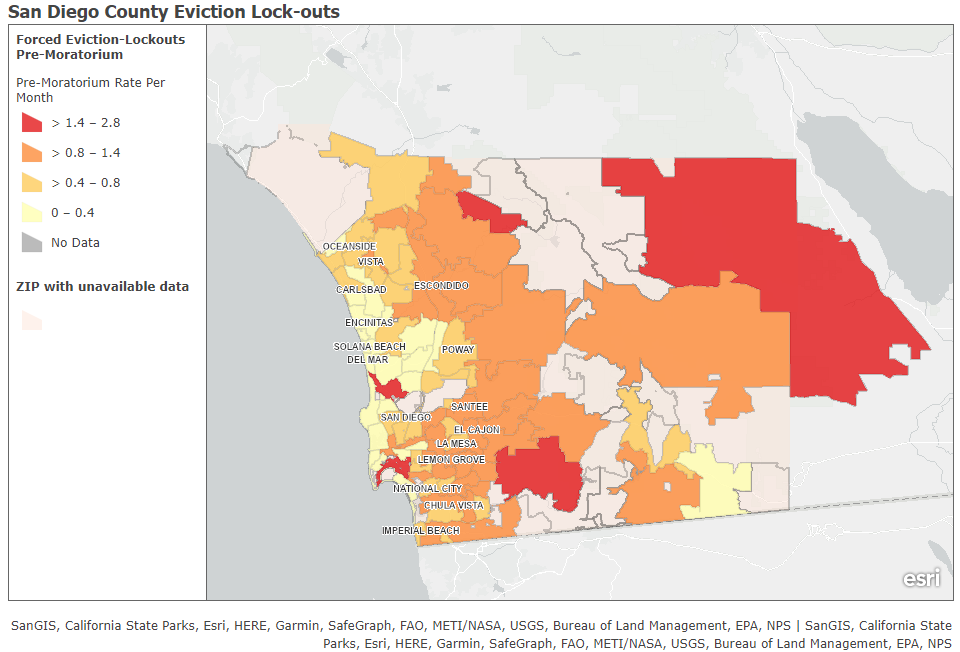
\includegraphics[width=\linewidth]{figures/gis_pre_figure1.png}
  \caption{Forced Lock-out Eviction orders in SD County before Moratorium.}
  \label{fig:ForcedEviction_BEFORE_fig1}
\end{figure}


It is interesting to note there are two coastal cities, Carlsbad and Oceanside, that are experiencing similar rates of eviction to inland areas. However, this changes when we look at during and after the moratorium and they continue to stay on the lower end of evictions just like the other coastal cities. This could be because these areas tend to hold different demographics from race/ethnicity, household income to rental costs. A 2022 Census estimate for Race and Hispanic Origin\footnote{These estimates to contain sampling errors but are useful in getting some understanding for city demographics \url{https://www.census.gov/quickfacts/fact/table/solanabeachcitycalifornia,encinitascitycalifornia,oceansidecitycalifornia,carlsbadcitycalifornia,sandiegocitycalifornia/PST045222}} demographics of several cities in San Diego County, California, highlight a diverse mix of residents. In Solana Beach, approximately 76\% of the population identifies as white alone, while the Hispanic/Latino community makes up around 17.4\% of the population. Moving to Encinitas, the majority of residents, approximately 82\%, identify as white alone, while the Hispanic/Latino population comprises about 16\% of the total. In Oceanside, the demographic landscape reveals a significant Hispanic/Latino presence, with approximately 61\% of the population identifying as such. White residents make up around 37.8\% of the population in Oceanside. Interestingly Carlsbad, similar to Solana and Encinitas, has a substantial white population, accounting for approximately 76\% of the residents. The Hispanic/Latino community represents around 15\% of the total population in Carlsbad. So why wouldn’t patterns of eviction for Carlsbad match areas with similar demographics? We do see that this area and Oceanside actually are starting to match the eviction patterns with their coastal city neighbors during and after the moratorium. 


\begin{figure}[H]
  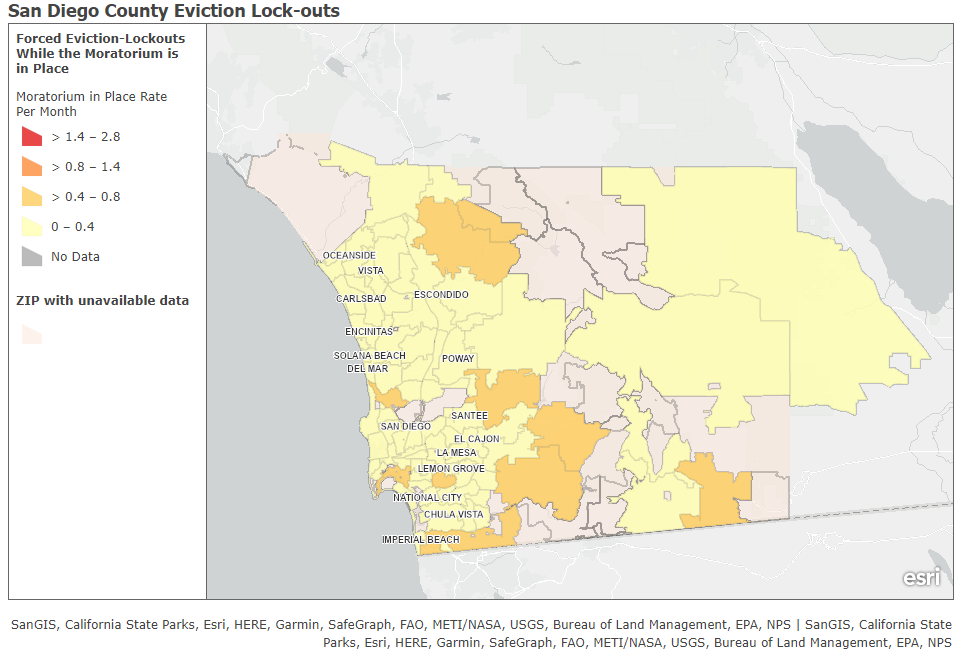
\includegraphics[width=\linewidth]{figures/gis_during_figure2.png}
  \caption{Forced Lock-out Eviction orders in SD County during Moratorium.}
  \label{fig:ForcedEvcitions_DURING_Fig2}
\end{figure}

We can see in figure \ref{fig:ForcedEvcitions_DURING_Fig2} that while the moratorium is in place there is a significant decrease in forced eviction rates. Some areas staying the same such as our coastal cities: Solana Beach, DelMar, and south coastal San Diego areas. In the previous map(see figure \ref{fig:ForcedEviction_BEFORE_fig1}) the further inland or east we went, eviction rates would increase. However, further inland we can see that these rates have dropped and are more uniform with a few areas having slightly high rates during the moratorium period. This is likely due to the eviction protections set in place during this time period. Areas we would expect to see having higher rates of eviction now have much lower instances of forced eviction due to the protections in place during this time period.

\begin{figure}[H]
  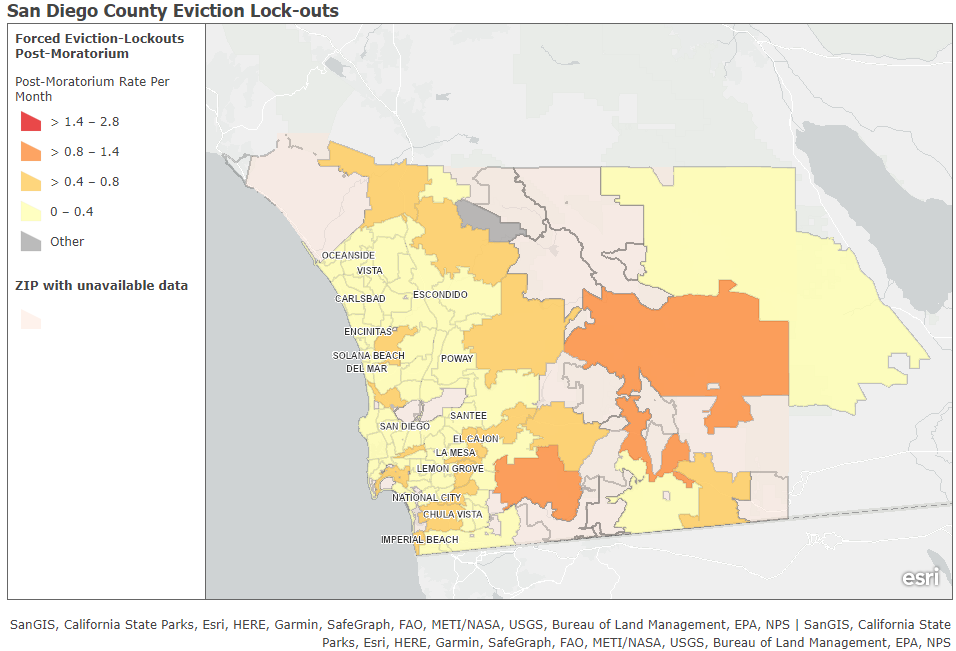
\includegraphics[width=\linewidth]{figures/gis_post_figure3.png}
  \caption{Forced Lock-out Eviction orders in SD County after Moratorium.}
  \label{fig:ForcedEvictions_AFTER_fig3}
\end{figure}
Once these moratoriums were lifted we expected to see a significant increase in eviction rates through the county. In figure \ref{fig:ForcedEvictions_AFTER_fig3} we can see that eviction rates are starting to increase beginning with the inland areas and a few southern cities. These patterns are consistent with the rates seen in figure \ref{fig:ForcedEviction_BEFORE_fig1}. Prior to the pandemic and the implementation of eviction protections, inland cities had higher eviction rates compared to central and coastal cities. This gives us concern that many people in these inland and southern areas will be faced with housing precarity following the moratorium ending, especially if San Diego county does regress back to higher rates of eviction. While our study only encompasses 9 months after the moratorium, the increase does seem to follow previous patterns of evictions in the county. To view these changes clearly in one graph we can refer to figure \ref{fig:ForcedEvcitions_DURING_Fig2} which shows us the Moratorium periods for the Covid-19 pandemic time frame: P1 = “Before-moratorium", P2 = “During Moratorium" and P3 = "After-moratorium". In this graph we can see the eviction rate for each period, calculated by month to better compare across the periods due to the differences in duration of each stage of the moratorium.


\begin{figure}[H]
  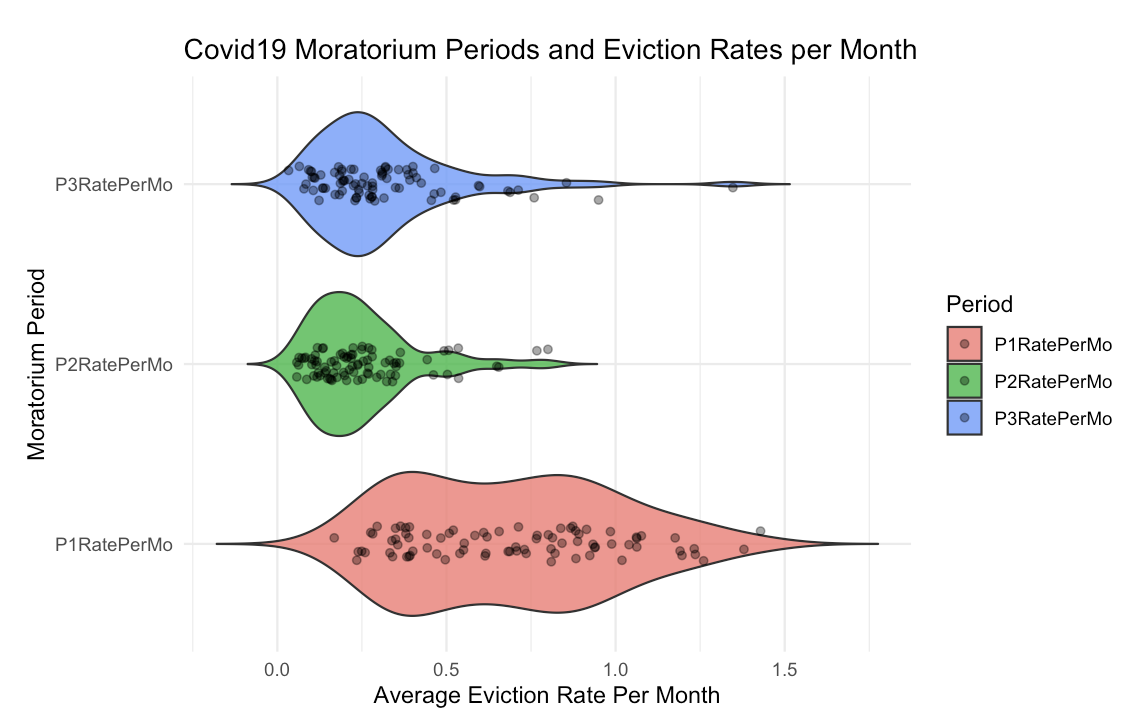
\includegraphics[width=\linewidth]{figures/Forced_EvictionRates_figure6.png}
  \caption{Illustrates the changes of eviction rate by month using a Violin plot. The colored area represents density and emphasizes any clustering patterns of eviction ZIP codes. To ensure the visualization is not skewed by outliers, only evictions that were within 2 standard deviations of the mean are included.}
  \label{fig:EvictionsRatesPerMonth_4}
\end{figure}

We can presume through this graph that rates of forced evictions are returning to what they were prior to the eviction protections being in place. In Period 1, eviction rates are more dispersed, indicating a wider range of evictions across ZIP codes. The density of data points is relatively uniform across the range of eviction rates in this period. In Period 2, which coincides with the moratorium, we observe less forced evictions with clustering of ZIP codes experiencing evictions at the lower end of the scale. As discussed previously in figure 2 this clustering closer to 0 eviction rate aligns with expectations during a moratorium period, where fewer evictions are expected to occur due to protections being in place. Finally in Period 3, we observe an elongation of the violin plot compared to Period 2, indicating an increase in forced eviction rates. The clustering of ZIP code evictions becomes more spread out in Period 3 compared to Period 2, suggesting a less concentrated distribution of eviction rates and the potential return to a pattern similar to what we see in Period 1. Additionally, there appears to be a slight increase in density along the tail of the plot in Period 3 which indicates ZIP codes moving toward an increase of  forced evictions.

These spatial analyses reveal notable differences between periods and regional differences. Further examination into these differences requires additional calculations. 

The following maps show the difference of eviction rate between the moratorium in place time frame and post-moratorium period. This difference is of interest because it highlights the time during and after the moratorium. It is important for us to explore how the end of the moratorium will affect eviction rates across San Diego County. Seeing as our prior analysis showed differences in coastal and inland regions, the objective is to conclude how much of a difference occurred in these areas(see figure 7). This map conveys the significant changes in forced eviction occurring between during and after the moratorium. Places such as ZIP codes 92036(Julian), 92131(San Diego), 92061(Pauma Valley), 91962(Pine Valley) all increased by 15\% or more in forced eviction-lockouts by the end of the moratorium. On the other hand, our coastal regions exhibited a decrease in eviction rates, such as Encinitas with a decrease of approximately 7\% followed by Oceanside(4\%), Del Mar(8\%), Solana Beach(8\%), and all the way down the San Diego coast decreasing at around the same frequency. Additionally, we can see that two areas, Bonsall and South Chula Vista, Imperial beach all saw a significant difference of a decrease in 24\% to 31\% less forced evictions. While our map showing forced evictions occuring after the moratorium(fig.5) provides a case for increasing rates of eviction in the inland and central areas of San Diego, we can see in figure 7 that these rates are supported by the findings in figure 5. Escondido had significantly increased by 20\% in forced eviction lockouts by the end of the moratorium and the surrounding areas saw an increase of 38\% or higher.


\begin{figure}[H]
  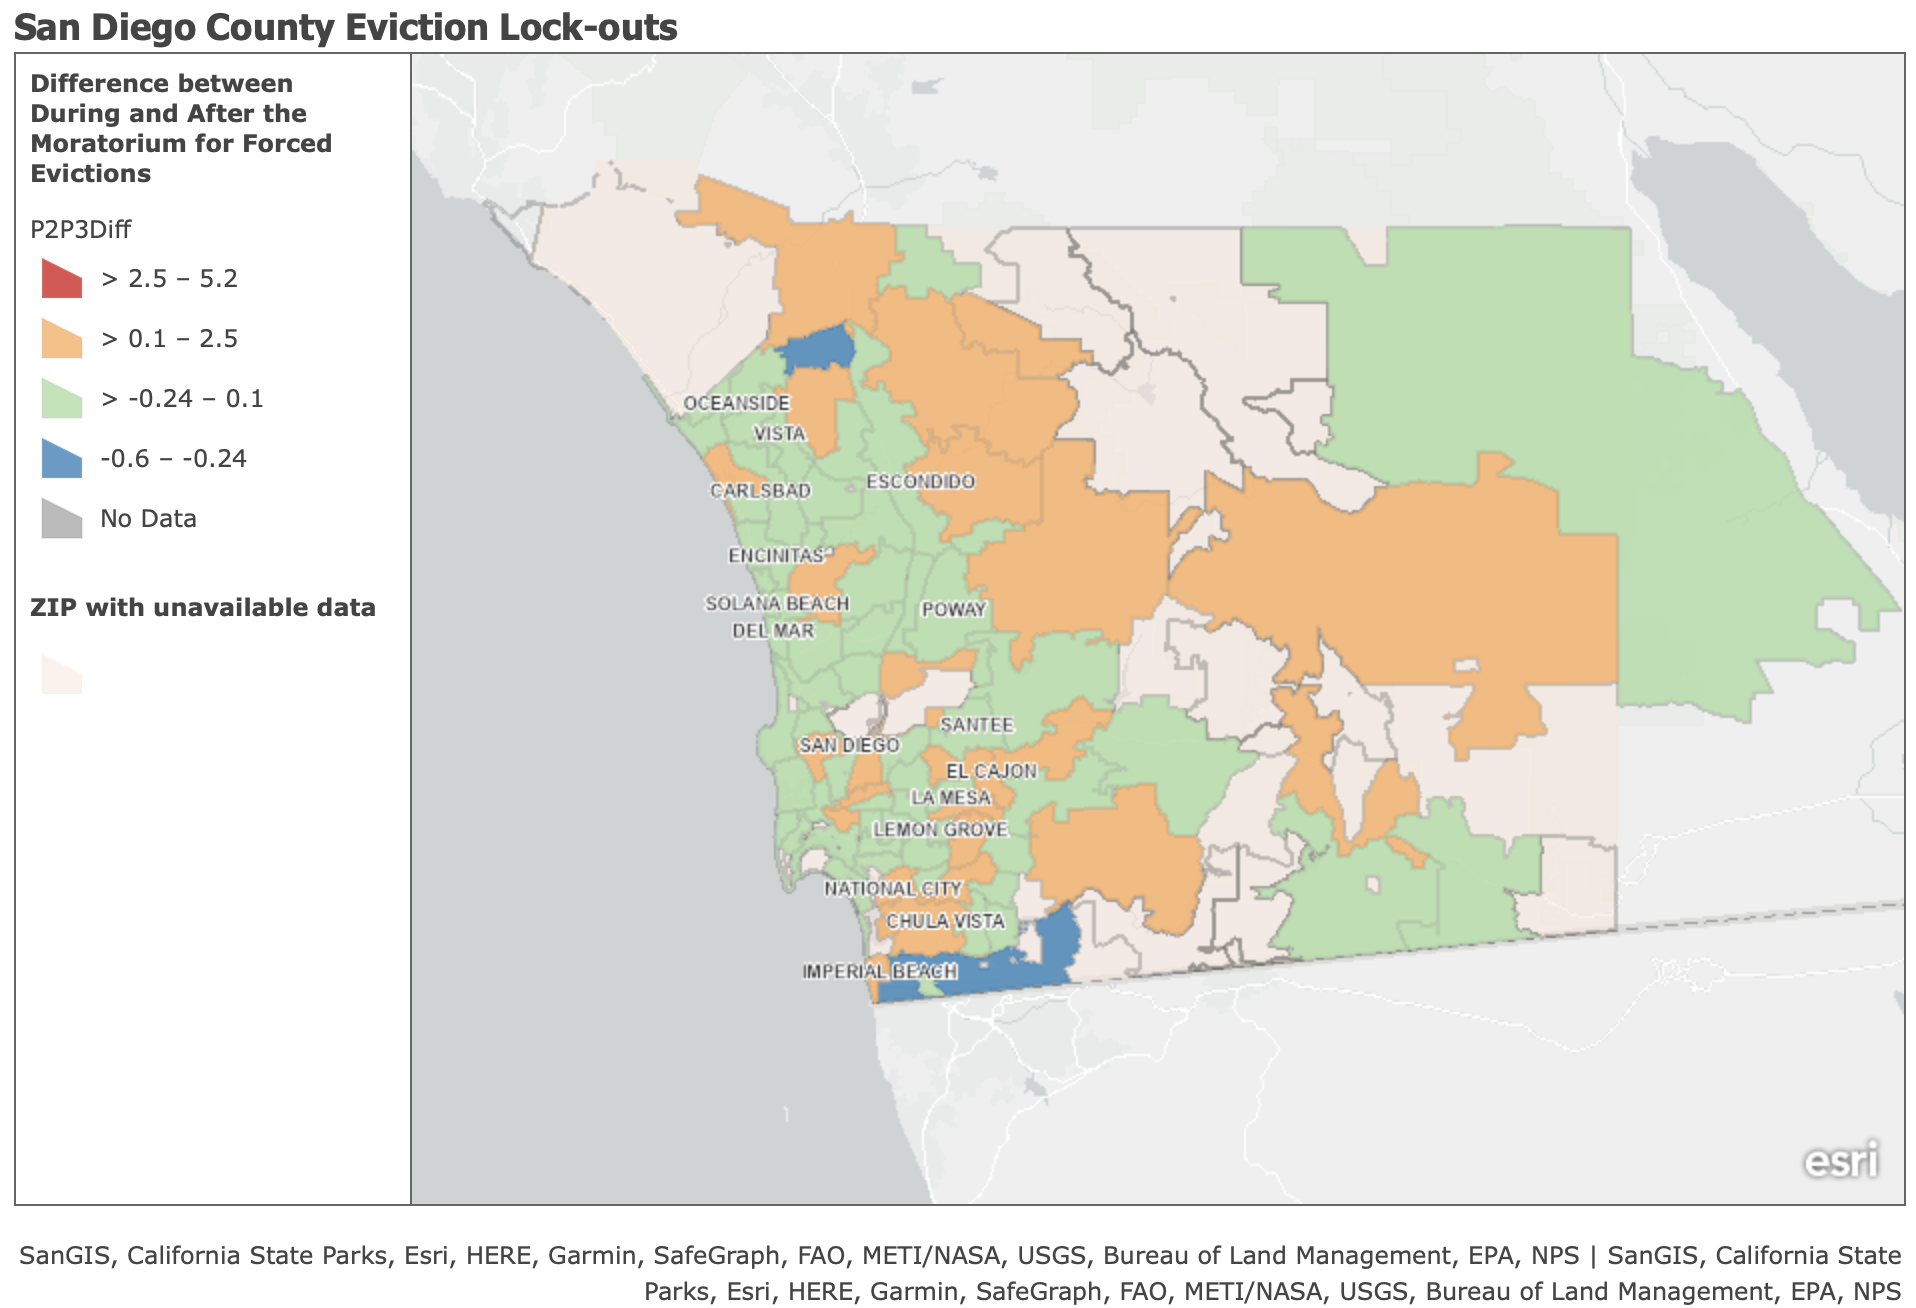
\includegraphics[width=\linewidth]{figures/gis_p2p3diff_figure4.png}
  \caption{Eviction Differences Between Periods.}
  \label{fig:Evictions_DuringtoPostMoratorium_5}
\end{figure}



\subsection{Statistical Analysis of Housing Instability in relation to San Diego County ZIP codes}


After conducting our in-sample analysis for both need outcomes indicating how likely one would have housing and/or utility needs, we found that while the standard errors\footnote{We utilize asymptotic standard error defined as $SE(\beta_i) = \sqrt{{(Variance \ Covariance \ Matrix)^{-1}_{ii}}}$} and effect sizes of p < 0.01 for both needs, we can derive from our in-sample model comparison criterion of AIC, that the added complexity when incorporating our alter models of adding in the moratorium effect leads to a model which is less likely to capture the changes occurring within the CIE demographic data when a need is determined per observation. In short, because the alternative models both receive an AIC score of = (42,199 \& 39,147) compared to the null model AIC scores of (27,328 \& 26,011) for an average reduction of model fit by 13,960, we have failed to reject the null hypothesis for our in-sample models indicating that while the effect sizes for our targeted covariates are strong, it does not improve the model fit overall and in fact reduces it by a large amount.

\begin{table}[!htbp] \centering 
  \caption{In-Sample Model Performance Scores: AIC/BIC lower is better | LogLik higher is better} 
  \label{} 
\begin{tabular}{@{\extracolsep{5pt}} cccc} 
\\[-1.8ex]\hline 
\hline \\[-1.8ex] 
 & AIC & BIC & LogLik \\ 
\hline \\[-1.8ex] 
Original Model $H_0$ (Housing Needs) & $27,328.6900$ & $27,415.7800$ & $$-$13,653.3400$ \\ 
Moratorium Added $H_1$ (Housing) & $42,199.7200$ & $42,286.8100$ & $$-$21,088.8600$ \\ 
Original Model $H_0$ (Utilities Needs) & $26,011.0100$ & $26,098.1000$ & $$-$12,994.5100$ \\ 
Moratorium Added $H_1$ (Utilities) & $39,060.9000$ & $39,147.9900$ & $$-$19,519.4500$ \\ 
\hline \\[-1.8ex] 
\end{tabular} 
\end{table}  


Having a poor model fit is indicative of the lack of fit for the moratorium period across both needs in capturing additional changes within the data, but it should be repeated that AIC only measures the fit in regards to model performance. Overall along with contextual understanding that predicting needs based off demographic data generated from 2-1-1 callers determined by CIE may potentially result in noisy data. In order to potentially filter out the noise (or variance) of the data, we can then look upon the out-of-sample performance which measures the discriminatory power of our categorical logit. As such, we look upon the area under the curve scores of all four models. We can see within Table 4 that all four models have slightly higher than chance predictive performance indicating all models overall perform poorly in capturing the data and ignoring noise. Furthermore, with the Moratorium Change covariate included in our alternative models, we do see a slight increase in performance for both needs, with the largest increase of 3.5\% predictive power for utilities needs.

\begin{table}[!htbp] \centering 
  \caption{AUC Scores for All Models, K = 50, R = 5} 
  \label{} 
\begin{tabular}{@{\extracolsep{5pt}} ccc} 
\\[-1.8ex]\hline 
\hline \\[-1.8ex] 
 & $H_0$ & $H_1$Moratorium Change Added \\ 
\hline \\[-1.8ex] 
Housing Needs & $0.5839$ & $0.5984$ \\ 
Utilities Needs & $0.6138$ & $0.6496$ \\ 
\hline \\[-1.8ex] 
\end{tabular} 
\end{table}  

What does this tell us overall? With an extremely large AIC increase for in-sample performance, it indicates that a categorical logistic regression is not necessarily the best method in capturing the CIE demographic data overall, and that the changes of Moratorium dates does not improve the model fit. Yet, with our out-of-sample performance measures, we can see that the predictive power of the models overall for the data do slightly increase when incorporating the Moratorium periods, we ultimately cannot reject the null hypothesis based on performance metric of $H_{1}AUC < 80\%$ when applying a categorical logistic regression.

\begin{figure}[H]
  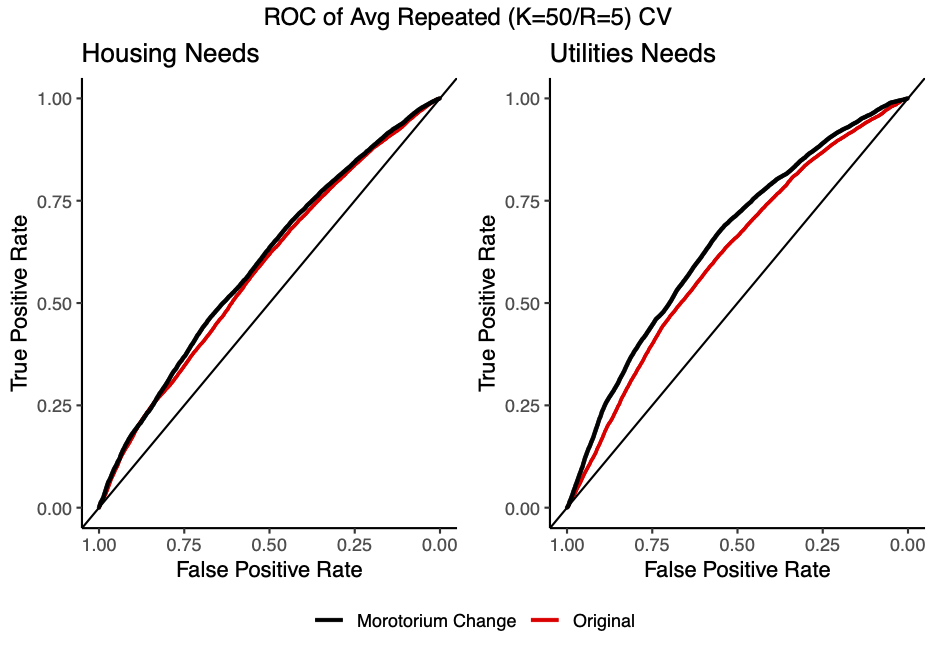
\includegraphics[width=\linewidth]{figures/auc_roc_out_of_sample.png}
  \caption{ROC/AUC Curve of Out-Of-Sample Model Performance for Logit Models | R = 5, K = 50.}
  \label{auc_roc_out_of_sample}
\end{figure}

This ended up being a surprise despite the failure to reject the null hypothesis regarding the CIE demographic data and the inability to derive any inferential claims from our fitted models, the greater than 60\% performance measure for Utilities Needs is telling on the complexity of the data as a whole. This tells us that further investigation into the dataset may necessitate a focus solely on utilities needs for an outcome predictor, and incorporating the Moratorium change, as well as a model which can better account for the noise within the data and more categorical predictors from the remaining variables within.


\begin{table}[H]
  \centering
  \resizebox{0.39\textwidth}{!}{%
    \begin{tabular}{@{\extracolsep{5pt}}lcc}
      \\[-1.8ex]\hline
      \hline \\[-1.8ex]
      & \multicolumn{2}{c}{\textit{Dependent variable:}} \\
      \cline{2-3}
      \\[-1.8ex] & Housing Needs & Utilities Needs \\
      \\[-1.8ex] & (1) & (2)\\
      \hline \\[-1.8ex]
      Female & 0.221$^{***}$ & 0.551$^{***}$ \\
      & (0.031) & (0.033) \\
      & & \\
      Age & $-$0.110$^{***}$ & 0.145$^{***}$ \\
      & (0.009) & (0.010) \\
      & & \\
      Alaska Native/Native Indian & $-$0.315$^{**}$ & $-$0.238$^{*}$ \\
      & (0.131) & (0.139) \\
      & & \\
      Asian/Pacific Islander/Hawaiian & $-$0.512$^{***}$ & $-$0.314$^{***}$ \\
      & (0.066) & (0.069) \\
      & & \\
      Bi-Racial/Multi-Racial & $-$0.345$^{***}$ & $-$0.169$^{**}$ \\
      & (0.073) & (0.077) \\
      & & \\
      Hispanic/Latino & $-$0.388$^{***}$ & $-$0.064 \\
      & (0.117) & (0.121) \\
      & & \\
      Race/Ethnicity: Other & $-$0.439$^{***}$ & 0.131$^{*}$ \\
      & (0.067) & (0.069) \\
      & & \\
      White/Caucasian & $-$0.508$^{***}$ & $-$0.402$^{***}$ \\
      & (0.040) & (0.042) \\
      & & \\
      White/Hispanic/Latino & $-$0.515$^{***}$ & $-$0.067 \\
      & (0.043) & (0.045) \\
      & & \\
      Poverty Percentage & 2.261$^{***}$ & 0.620 \\
      & (0.499) & (0.519) \\
      & & \\
      During Moratorium & $-$0.156$^{***}$ & $-$0.591$^{***}$ \\
      & (0.031) & (0.033) \\
      & & \\
      Post-Moratorium & $-$0.710$^{***}$ & $-$1.137$^{***}$ \\
      & (0.055) & (0.062) \\
      & & \\
      Constant & 0.310$^{***}$ & $-$0.944$^{***}$ \\
      & (0.063) & (0.066) \\
      & & \\
      \hline \\[-1.8ex]
      Observations & 20,282 & 20,282 \\
      \hline
      \hline \\[-1.8ex]
      \textit{Note:} & \multicolumn{2}{r}{$^{*}$p$<$0.1; $^{**}$p$<$0.05; $^{***}$p$<$0.01} \\
    \end{tabular}%
  }
  \caption{Likelihood table of Housing Needs and Utilities Needs, factored by race and Moratorium Period. (Constant indicates when both race/ethnicity and moratorium are at their reference levels)}
  \label{}
\end{table}






\section{Discussion}

Studying housing instabilities and eviction can be complex and tricky due to legal aspects, unavailability of data, and consistency of good data\parencite{Cheng2021}. Our research contributes to the scholarly understanding of housing instability by drawing on two types of housing-related data that cover a time period that includes state eviction moratoria. We saw through this study that eviction rates are increasing. From during the moratorium period to after we found forced eviction lock-outs increased by 20\% or more. It's important we continue to be aware of the implications of removing the moratorium, especially for those who are experiencing instability. We can see from our results that the patterns of eviction after the moratorium period look to be returning to similar patterns as before the moratorium period. An increase of evictions is occurring starting with inland areas of San Diego County and if these patterns continue we could see eviction rates return to what they were prior to the moratorium. It is important that we focus our attention on these areas and understand why the inland cities tend to experience higher eviction rates than their coastal counterparts. 

Finding explanations for housing precarity or security can be done through models tested on eviction, but not on CIE data. Based on our findings utilizing eviction rate, we can see that the rate of evictions during the moratorium reversed. Yet, when utilizing CIE 2-1-1 demographic data, we see a slight increase in model performance when incorporating Moratorium on predicting housing precarity, but a stark decrease in model fit. Further research on this issue can be justified in order to better understand what additional fail safes have assisted individuals in staying secure during the COVID-19 pandemic. Did the stimulus have an effect during this time? Was there a rise in program assistance sign-ups? Did employment play any role? According to our data, while employment did not explain our models well, we did find that household income was a good fit for understanding housing insecurity.

Overall, the study's findings indicate clear differences in eviction rates and changes in housing security before, during, and after the Covid-19 Moratorium for San Diego County. The temporal dynamics analysis revealed shifts in eviction trends and patterns during these periods. The models revealed the best variables that explain housing instability or in contrast housing security had significant effects during the moratorium periods. 

Further steps to move forward with this data could be possible imputations in order to preserve more than the 20\% of data this study was able to work with. Exploring models which can better capture the CIE 2-1-1 demographic data through the noise present, focusing on utility needs solely when researching demographic trends for 2-1-1 calls, as well as investigating qualitative aspects of the effects of the moratorium on members within San Diego County for their own personal insights on the topic.

% we're at the end of the paper here, so just print the bibliography
\printbibliography[]
\end{document}